\apendice{Especificación de diseño}
\section{Clasificación de las asignaturas}
Se ha realizado una clasificación general de las áreas a las que pertenecen de forma general las  asignaturas, de forma que se pueda mostrar un gráfico en la materia recomendable para un alumno. La siguiente tabla hace referencia a dicha clasificación \ref{tab:1}
\begin{table}[]
\caption{Tabla áreas educativas de las asignaturas }
\label{tab:1}
\resizebox{\textwidth}{!}{
\begin{tabular}{ lrrrrrrrr }
\toprule
 & Matemáticas & Derecho & Programación & Algoritmos & Idiomas & Economía & Diseño & Equipos informáticos \\  
\textbf{PRIMER SEMESTRE} &  &  &  &  &  &  &  &  \\  
Fundamentos Deontológicos y Jurídicos de las TIC & 1 & 1 & 0 & 0 & 0 & 0 & 0 & 0 \\  
Álgebra Lineal & 1 & 0 & 0 & 0 & 0 & 0 & 0 & 0 \\  
Informática Básica & 0 & 0 & 1 & 0 & 0 & 0 & 0 & 0 \\  
Fundamentos Físicos de la Informática & 1 & 0 & 0 & 0 & 0 & 0 & 0 & 0 \\  
Matemática Discreta & 1 & 0 & 0 & 0 & 0 & 0 & 0 & 0 \\  
\textbf{SEGUNDO SEMESTRE} &  &  &  &  &  &  &  &  \\  
Inglés Aplicado a la Informática & 0 & 0 & 0 & 0 & 1 & 0 & 0 & 0 \\  
Cálculo & 1 & 0 & 0 & 0 & 0 & 0 & 0 & 0 \\  
Programación & 0 & 0 & 1 & 1 & 0 & 0 & 0 & 0 \\  
Fundamentos de los Computadores & 0 & 0 & 1 & 0 & 0 & 0 & 0 & 1 \\  
Sistemas Operativos & 0 & 0 & 1 & 1 & 0 & 0 & 1 & 1 \\  
\textbf{TERCER SEMESTRE} &  &  &  &  &  &  &  &  \\  
Metodología de la Programación & 0 & 0 & 1 & 1 & 0 & 0 & 0 & 0 \\ 
Estadística & 1 & 0 & 0 & 0 & 0 & 0 & 0 & 0 \\ 
Ingeniería del Software & 0 & 0 & 0 & 0 & 0 & 0 & 1 & 0 \\  
Bases de Datos & 0 & 0 & 1 & 0 & 0 & 0 & 1 & 0 \\  
Arquitectura de Computadores & 0 & 0 & 1 & 0 & 0 & 0 & 0 & 1 \\  
\textbf{CUARTO SEMESTRE} &  &  &  &  &  &  &  &  \\  
Estructuras de Datos & 0 & 0 & 1 & 1 & 0 & 0 & 0 & 0 \\  
Redes & 0 & 0 & 0 & 0 & 0 & 0 & 0 & 1 \\  
Interacción Hombre-Máquina & 0 & 0 & 1 & 0 & 0 & 0 & 1 & 0 \\  
Fundamentos de Organización y Gestión de Empresas & 0 & 0 & 0 & 0 & 0 & 1 & 0 & 0 \\  
Análisis y Diseño de Sistemas & 0 & 0 & 0 & 0 & 0 & 0 & 1 & 0 \\  
\textbf{QUINTO SEMESTRE} &  &  &  &  &  &  &  &  \\ 
Arquitecturas Paralelas & 0 & 0 & 1 & 0 & 0 & 0 & 0 & 1 \\ 
Sistemas Inteligentes & 0 & 0 & 1 & 1 & 0 & 0 & 1 & 0 \\ 
Gestión de Proyectos & 0 & 0 & 1 & 0 & 0 & 1 & 1 & 0 \\ 
Diseño y Administración de Sistemas y Redes & 0 & 0 & 0 & 0 & 0 & 0 & 0 & 1 \\  
Procesadores del Lenguaje & 0 & 0 & 1 & 1 & 0 & 0 & 0 & 0 \\  
\textbf{SEXTO SEMESTRE} &  &  &  &  &  &  &  &  \\ 
Programación Concurrente & 0 & 0 & 1 & 0 & 0 & 0 & 0 & 1 \\  
Seguridad Informática & 0 & 1 & 1 & 1 & 0 & 0 & 0 & 1 \\ 
Aplicaciones de Bases de Datos & 0 & 0 & 1 & 0 & 0 & 0 & 1 & 1 \\  
Algoritmia & 0 & 0 & 1 & 1 & 0 & 0 & 0 & 0 \\ 
Métodos Numéricos y Optimización & 1 & 0 & 1 & 0 & 0 & 0 & 0 & 0 \\  
\textbf{SÉPTIMO SEMESTRE} &  &  &  &  &  &  &  &  \\  
Diseño e Implementación de Sistemas Digitales & 0 & 0 & 1 & 0 & 0 & 0 & 1 & 1 \\ 
Gestión de la Información & 1 & 0 & 1 & 1 & 0 & 1 & 0 & 0 \\ 
Diseño y Mantenimiento del Software & 0 & 0 & 1 & 0 & 0 & 0 & 1 & 0 \\  
Organización y Gestión de Empresas & 0 & 0 & 1 & 1 & 0 & 1 & 0 & 0 \\  
 Mantenimiento de Equipos Informáticos & 1 & 0 & 0 & 0 & 0 & 0 & 0 & 1 \\  
Hardware de Aplicación Específica & 0 & 0 & 1 & 0 & 0 & 0 & 1 & 1 \\ 
Control por Computador & 0 & 0 & 1 & 0 & 0 & 0 & 0 & 1 \\ 
Validación y Pruebas & 0 & 0 & 1 & 1 & 0 & 0 & 1 & 0 \\
Computación Neuronal y Evolutiva & 0 & 0 & 1 & 1 & 0 & 0 & 0 & 0 \\ 
Programación de Sistemas Operativos & 0 & 0 & 1 & 0 & 0 & 0 & 0 & 1 \\ 
\textbf{OCTAVO SEMESTRE} &  &  &  &  &  &  &  &  \\ 
Sistemas Distribuidos & 0 & 0 & 1 & 1 & 0 & 0 & 1 & 0 \\ 
Sistemas Empotrados y de Tiempo Real & 0 & 0 & 1 & 0 & 0 & 0 & 0 & 1 \\
Métodos Formales & 1 & 0 & 1 & 0 & 0 & 0 & 1 & 0 \\ 
Nuevas Tecnologías y Empresa & 0 & 0 & 1 & 1 & 0 & 0 & 0 & 0 \\ 
Minería de Datos & 1 & 0 & 1 & 1 & 0 & 0 & 0 & 0 \\ 
Desarrollo Avanzado de Sistemas Software & 0 & 0 & 1 & 0 & 0 & 0 & 1 & 0 \\ \bottomrule
\end{tabular}
}
\end{table}


\section{Modelo de Interfaz Gráfica}
La interfaz gráfica de escritorio de la primera versión se realizará con PyQt5, de forma que habrá varias ventanas diferentes dependiendo de la funcionalidad seleccionada: 
\subsection{Inicio de Sesión}
En la primera pestaña al ejecutar la aplicación, se mostraría la pantalla de inicio sesión para introducir el correo y la contraseña. La siguiente imagen hace referencia a un modelo básico de la pantalla de inicio de sesión. ~\ref{fig:C.1}
\begin{figure}[h]
\centering
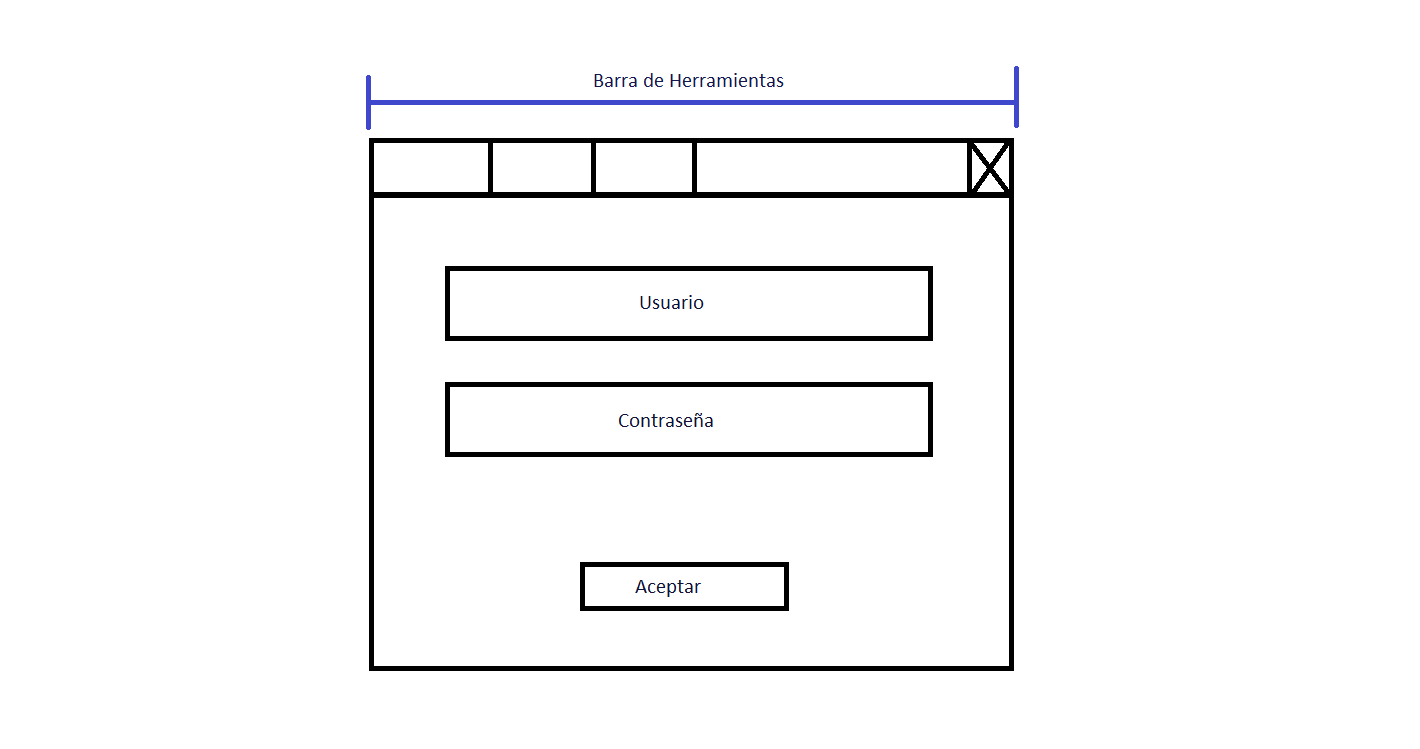
\includegraphics[width=0.90\textwidth]{PROTOTIPO_Inicio_sesion}
\caption{Prototipo de Inicio Sesión}
\label{fig:C.1}
\end{figure}

\subsection{Rellenado de cuestionario}
Una vez registrado por primera vez, un usuario debe rellenar el cuestionario con las ponderaciones de las asignaturas cursadas. Esta pestaña también sirve en caso de que el usuario se haya confundido en la calificación de alguna asignatura o repita el sistema de recomendación tras cursar nuevas asignaturas. Los diferentes cursos se seleccionarán en los botones para evitar un exceso de asignaturas mostradas en la pestaña. La siguiente imagen hace referencia a dicha pestaña. ~\ref{fig:C.2}
\begin{figure}[h]
\centering
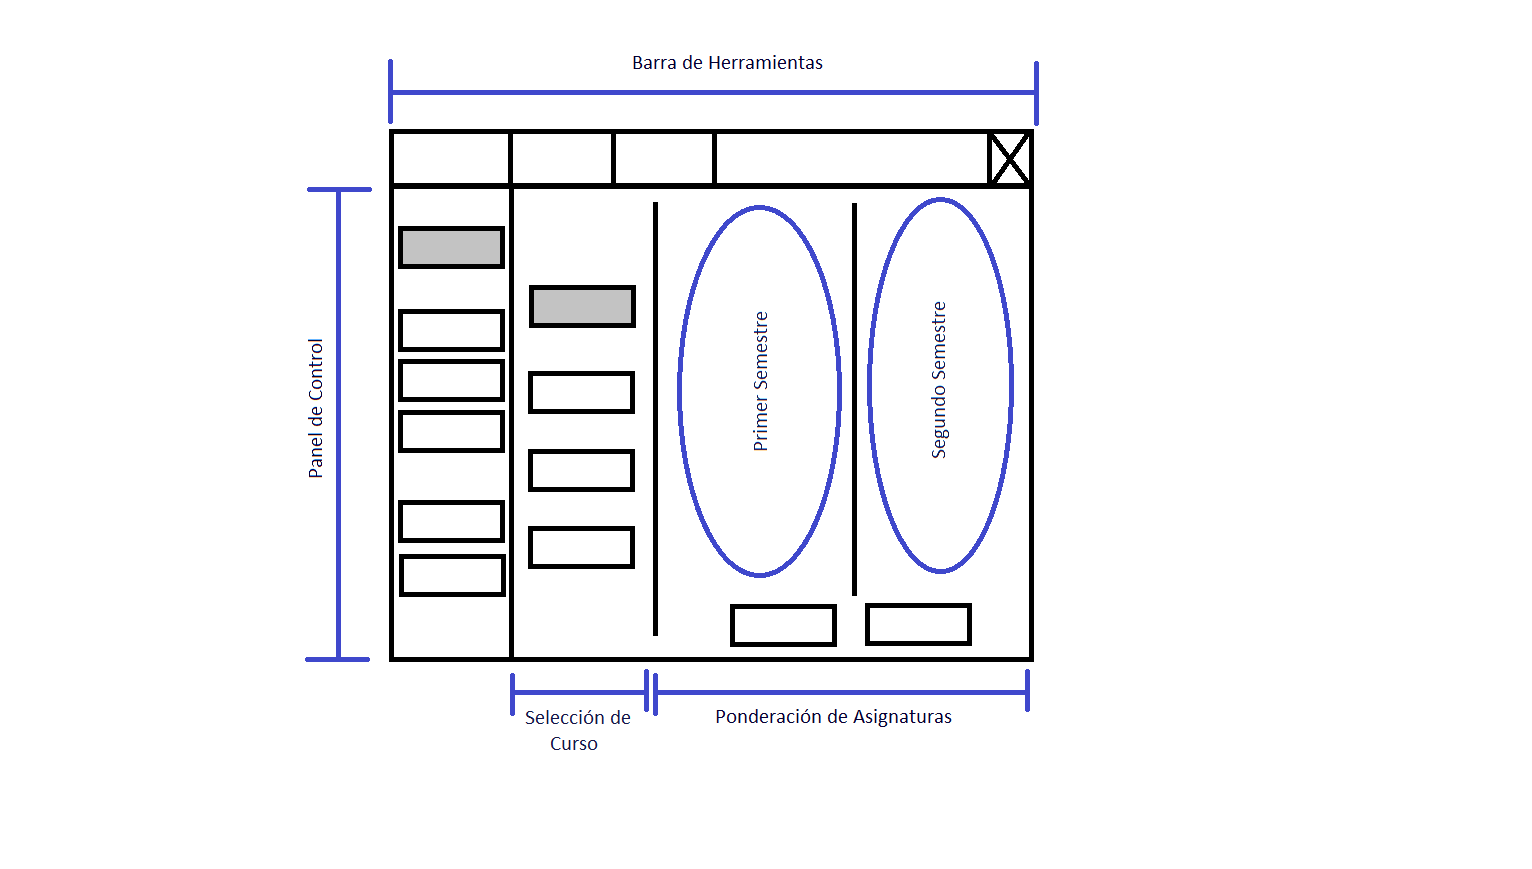
\includegraphics[width=0.90\textwidth]{PROTOTIPO_Rellenado_Datos}
\caption{Prototipo de Rellenado de datos}
\label{fig:C.2}
\end{figure}
\subsection{Muestra de resultados}
Tras rellenar el cuestionario para la recogida de datos, se seleccionará el sistema de recomendación deseado, y se mostrarán los resultados en base al sistema seleccionado, teniendo como patrón en el centro de la ventana los resultados de las asignaturas no cursadas, y en el tercio derecho, se mostrarán unas gráficas de las asignaturas y preferencias del alumno. La siguiente imagen hace referncia a dicha pestaña: ~\ref{fig:C.3}
\begin{figure}[h]
\centering
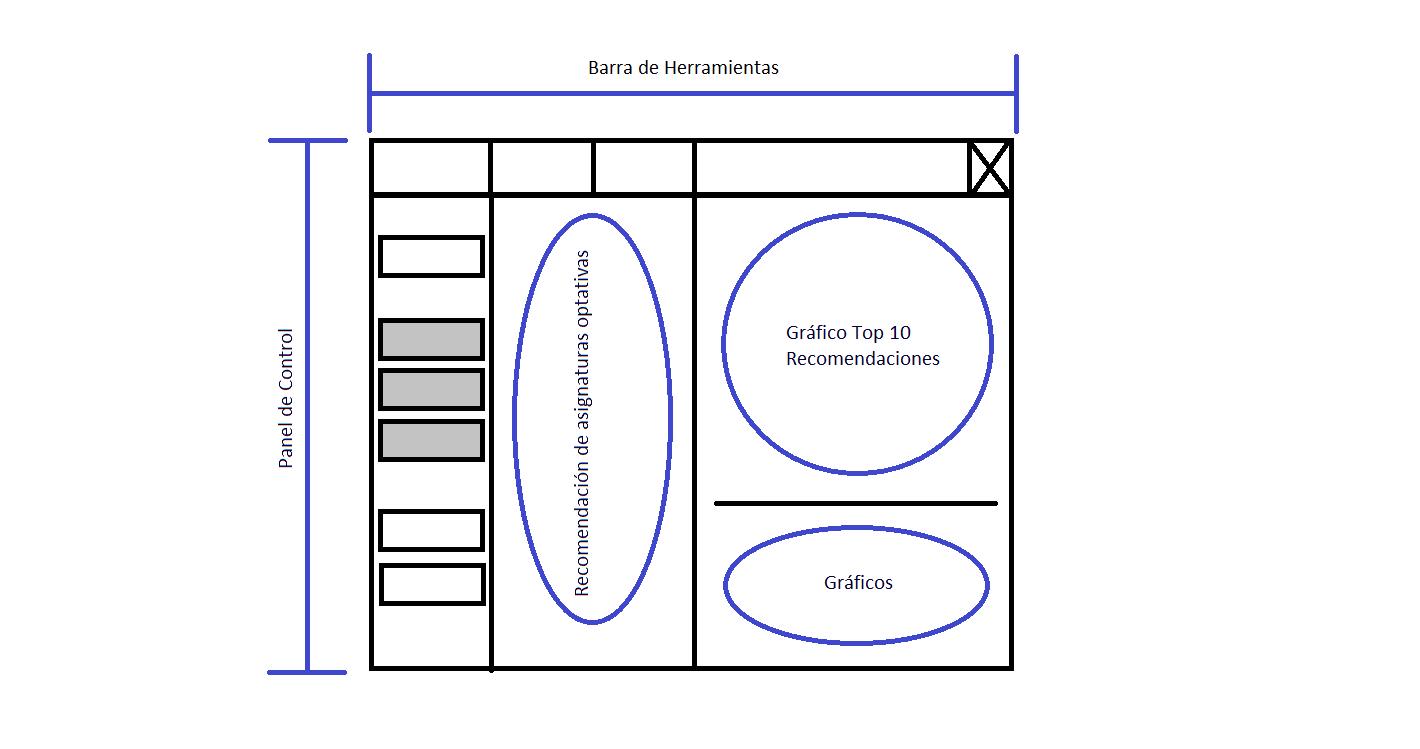
\includegraphics[width=0.90\textwidth]{PROTOTIPO_Sistemas_Recomendacion}
\caption{Prototipo de la muestra de datos}
\label{fig:C.3}
\end{figure}

\subsection{Otros datos}
Habrá un botón adicional que muestre las preferencias generales de media de los usuarios, así como otras gráficas para información adicional al usuario. 
La siguiente imagen hace referencia a dicha pestaña: ~\ref{fig:C.4}
\begin{figure}[h]
\centering
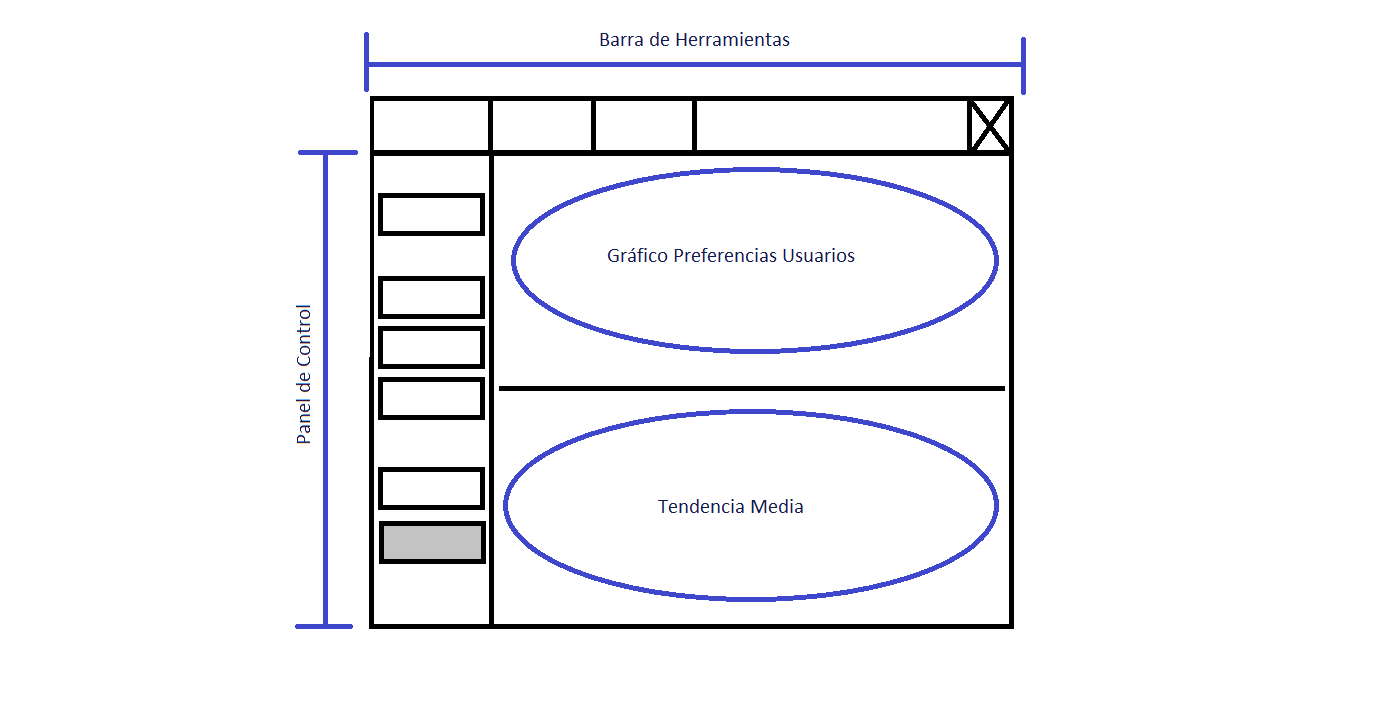
\includegraphics[width=0.90\textwidth]{PROTOTIPO_Otros_Datos}
\caption{Prototipo de datos adicionales}
\label{fig:C.4}
\end{figure}
